\documentclass{standalone}
\usepackage{tikz}
\begin{document}
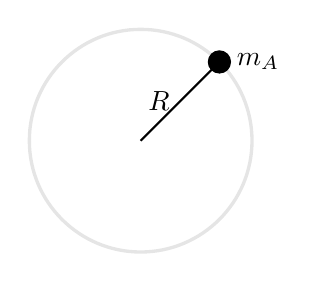
\begin{tikzpicture}
    %\node[] at (0,1.7) {\small{$\delta h_{+,\times}(t)\approx A_{GR}(t) \exp\left(i\delta\Psi_{vis} t\right)$}};
    \filldraw[color=black!10, fill=white, very thick](0,0) circle (1.414);
    %\draw[thick    ] ( 0, 0) -- node[above left] {\small{$r$}} ++ (1,1);
    \filldraw[black, thick] ( 0, 0) -- (1, 1) node[midway,left] {\textcolor{black}{$R$}};
    \filldraw[black] ( 1, 1) circle (4pt) node[right] { $\;m_A$};
    \end{tikzpicture}
\end{document}

